\documentclass[a4paper,10pt]{article}

\usepackage[spanish]{babel} % Se selecciona el español como el idioma principal
\usepackage[utf8]{inputenc}
\usepackage{bookman}
\usepackage{color} % Paquete de color
\usepackage{graphicx,wrapfig} % Paquete de gráficos
\usepackage{anysize}
\usepackage[pdftex=true,colorlinks=true,linkcolor=black,urlcolor=blue,bookmarksopen=true]{hyperref}
\usepackage{bookmark}
\usepackage{enumitem,pifont}
\usepackage{amssymb,amsmath,mathtools,cancel,centernot}
\usepackage[dvipsnames]{xcolor}

\begin{document}

\newcommand{\HRule}{\rule{\linewidth}{0.5mm}}

\begin{figure}[t]
\begin{center}
    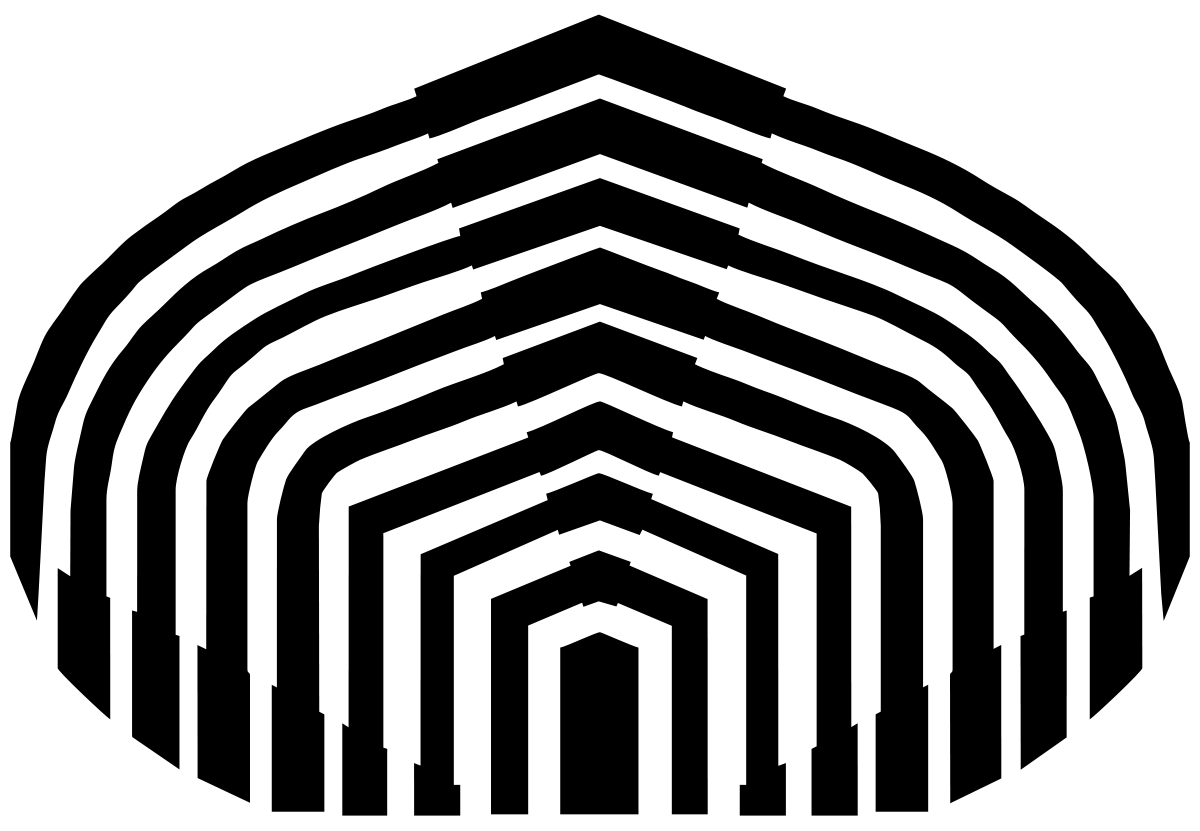
\includegraphics[scale=0.07]{USB.png}\\[0.6cm]
    \textsc
    {
        \LARGE Universidad Simón Bolívar \\[0.5cm]
    }
    \HRule \\[0.4cm]
    {\huge \bfseries Unidad 0: Campo Magnético} \\[0.4cm]
    
    Junior Zambrano\\[0.05cm]
    e-mail: 18-10929@usb.ve\\[0.2cm]
    \textsc{
    Octubre de 2021
    }
\end{center}
\end{figure}

% ----------------------------------------------------------------------
% ----------------------------------------------------------------------

\section*{Introducción}

El presente es un compendio teórico de la unidad de repaso del curso
\textbf{Física 4 (FS-2212)} que trata del campo magnético. Este resumen
fue elaborado a partir de apuntes, notas y síntesis de
las clases dictadas por el profesor \textbf{Sttiwuer Díaz} mientras impartía
dicho curso durante el trimestre virtual \textbf{Enero-Marzo 2021}.

Cualquier error y/o sugerencia, por favor notificar al autor de este documento.

\renewcommand{\labelitemi}{\ding{226}}
\renewcommand{\labelitemii}{\ding{226}}
\renewcommand{\labelitemiii}{\ding{226}}
\renewcommand{\labelitemiv}{\ding{226}}

% ----------------------------------------------------------------------
% ----------------------------------------------------------------------

% Clase 1

\section{Magnetismo y teoría electomagnética}

% ----------------------------------------------------------------------

\subsection{Línea de tiempo del magnetismo}

\begin{itemize}
    
\item 800 a.C.: Descubrimiento de la magnetita.

    \begin{itemize}
    
    \item La magnetita es un mineral de hierro constituido por óxido ferroso
    ($\text{Fe}_3\text{O}_4$), capaz de atraer otros metales hacia sí misma.
    
    \item Los materiales con esta propiedad recibieron el nombre de imán.
    
    \item Los imanes pueden ser:
    
        \begin{itemize}
        
        \item Naturales o permanentes: materiales compuestos de óxido ferroso.
        
        \item Inducidos: son construidos con materiales metálicos y tienen propiedades
        similares a la magnetita. 
        
        \end{itemize}
    
    \end{itemize} 

\item 1100: Aparición de la brújula.

    \begin{itemize}
    
    \item Una brújula es un instrumento que utiliza una aguja imantada por inducción que,
    al dejarse rotar libremente, se orienta a una determinada dirección si se acerca a
    un imán permanente.
    
    \item Fue descrita formalmente por primera vez por el matemático chino Sken Kua.

    \end{itemize}

\item 1269: Líneas de campo magnético.

    \begin{itemize}
    
    \item Petrus Peregrinus de Maricourt
    
        \begin{itemize}
        
        \item Las direcciones en las que apunta una aguja magnetizada en la cercanía
        de un imán (el imán utilizado fue uno esférico), las líneas bordeaban
        dicho imán y se hacían más intensas en los puntos extremos.
        
        \item El aspecto más relevante de este descubrimiento es que todo imán,
        independientemente de la forma que tenga, presenta dos polos (los
        cuales fueron llamados norte y sur) cuyas líneas de campo se orientan
        desde el polo norte al polo sur.
        
        \item Todas las líneas de campo magnético son líneas cerradas (conectadas).
        
        \item Esto implica que las fuentes de campo magnético no presentan
        flujo sobre superficies cerradas. La razón es porque la cantidad de líneas
        de campo que entran en dicha superficie coincide con la misma cantidad de líneas que
        salen de ella. Esto se conoce como la ley de Gauss magnética y se expresa:

        \begin{equation*}
            \boxed{
            \oint\vec{B}\cdot\hat{n}\mathrm{d}A=0
            }
            \text{ (forma integral)}
            \Longleftrightarrow
            \boxed{
            \vec{\nabla}\cdot\vec{B}=0
            }
            \text{ (forma diferencial)}
        \end{equation*}
        
        \end{itemize}
    
    \end{itemize}

\item 1600: Interacción magnética.

    \begin{itemize}

    \item Sir William Gilbert
    
        \begin{itemize}
        
        \item Establece que polos iguales se repelen y polos diferentes se atraen.
        
        \item La tierra se comporta como una gran imán.
    
        \item Nota: las brújulas apuntan hacia el polo sur magnético ($S_m$)
        de la tierra, que corresponde al polo norte geográfico ($N_g$).

        \end{itemize}

    \end{itemize}

\item 1750: Fuerza magnética.

    \begin{itemize}
    
    \item John Mitchell
    
        \begin{itemize}
        
        \item Establece que en una región hay un campo magnético cuando se manifiestan acciones
        magnéticas sobre imanes.
    
        \end{itemize}

    \end{itemize}

\item 1819: Electridad y magnetismo

    \begin{itemize}    
    
    \item Christian Oersted
    
        \begin{itemize}
            
        \item Establece que las interacciones magnéticas son generadas por cargas en movimiento
        (corrientes).
        
        \end{itemize}
            
    \end{itemize}

\item 1820: Ley de Biot-Savart

    \begin{itemize}

    \item Biot y Savart hacen una caracterización completa de como serían las líneas de campo
    generadas por alambres con corriente eléctrica.   
    
    \item Expresión matemática de la Ley de Biot-Savart-Laplace:
    
    \begin{equation*}
        \vec{B}(\vec{r})=\frac{\mu_0 I}{4\pi}
        \int \frac{\mathrm{d}\vec{\ell}\times\hat{r}}{r^2}
    \end{equation*}
    
\end{itemize}

\item 1826: Nacimiento de la Electrodinámica

    \begin{itemize}
        
    \item André-Marie Ampère
    
        \begin{itemize}
            
        \item Presenta su trabajo de electrodinámica, donde establece que
        los alambres con corriente interactúan magnéticamente entre sí.

        \item Explica el magnetismo en la materia mediante corrientes
        moleculares.

        \item Un cuerpo no magnetizado presenta corrientes dispuestas en
        forma aleatoria donde su efecto se neutraliza.

        \end{itemize}
    
    \end{itemize}

\item 1831: Inducción magnética

    \begin{itemize}
    
    \item Henry, Faraday y Lenz descubrieron casi de forma independiente
    la ley de inducción magnética que establece:

    El magnetismo puede aparecer variando el flujo de campo magnético
    sobre una espira, induciendo con ello corrientes eléctricas o fem
    (fuerzas electromotriz).

    \begin{equation*}
        \varepsilon = -\frac{\mathrm{d}\Phi_B}{\mathrm{d}t}
        \quad
        \Phi_B=\int\vec{B}\cdot\hat{n}\mathrm{d}a
    \end{equation*}

    \end{itemize}

\item 1873: Electromagnetismo

    \begin{itemize}
        
    \item James Clerk Maxwell

        \begin{itemize}
            
        \item Teoría o conjunto de leyes que unifican la electricidad y el
            magnetismo.
            
        \item Son tres los principales grupos en los que se divide el electromagnetismo: 
            
            \begin{itemize}
                
            \item Electrostática:
            
                \begin{enumerate} 
                    
                \item Búsqueda de campos eléctricos a partir de
                    cargas en reposo. 
                    
                \item Determinar la fuerza eléctrica que se
                ejercen sobre cargas en reposo o movimiento.
                
                \item Los campos son independientes del tiempo.
                
                \end{enumerate}

            \item Magnetostática:
            
                \begin{enumerate}
                    
                \item Búsqueda de campos magnéticos a partir de
                cargas en movimiento.
                
                \item Determinar la fuerza magnética que se
                ejercen sobre cargas en movimiento.
                
                \item Los campos son independientes del tiempo.
                
                \end{enumerate}
            
            \item Electrodinámica:
            
                \begin{enumerate}
                
                \item Búsqueda de campos eléctricos y magnéticos dependientes
                del tiempo generadas por diversas fuentes de carga o corrientes.
                
                \item Determinar la fuerza de Lorentz (suma de la fuerza
                eléctrica más la fuerza magnética) o fuerzas de distribuciones
                de cargas.
                
                \begin{equation*}
                    \boxed{\vec{F}=q(\vec{E}+\vec{v}\times\vec{B})}
                \end{equation*}

                \item Generación de ondas electromagnéticas.
                
                \end{enumerate}

            \end{itemize}
        
        \end{itemize}
        
    \end{itemize}
    
\end{itemize}
% ----------------------------------------------------------------------

\subsection{Imanes permanentes}

\begin{itemize}
    
\item Los polos magnéticos de los imanes siempre ocurren por pares
y no es posible aislarlos.

Esto quiere decir que si divido un imán a la mitad se producen dos
imanes con dos polos magnéticos cada uno.

\item No hay evidencia experimental de los monopolos magnéticos.

\end{itemize}

% ----------------------------------------------------------------------

\subsection{Fuerza magnética}

\begin{itemize}
    
\item Si se coloca una partícula cargada $q$ dentro de un campo magnético,
se obtienen los siguientes resultados:

    \begin{itemize}
        
    \item La magnitud de la fuerza magnética es proporcional a la carga
    $q$ de la partícula.

    \item La magnitud de la fuerza magnética es proporcional a la magnitud de
    campo magnético $B$.

    \item La fuerza magnética depende de la velocidad de la partícula.
    
    \item La fuerza magnética $\vec{F_B}$ es siempre perpendicular a $\vec{B}$
    y a $\vec{v}$.

    De manera que si la partícula se mueve en dirección del campo, lo que
    voy a obtener es que sobre la partícula no actúa ninguna fuerza magnética.

    \end{itemize}

\item \label{F_B} La expresión matemática de la fuerza magnética sobre una partícula
de carga $q$ y masa $m$ que se mueve con una cierta velocidad $\vec{v}$
inmersa en una región de campo magnético $\vec{B}$ puede describirse como:

\begin{equation*}
    \boxed{
    \vec{F}_{B}=q\vec{v}\times\vec{B}
    }
\end{equation*}

En conclusión:

\begin{equation*}
    \boxed{
    \left\lvert\vec{F}_{B}\right\rvert
    =\left\lvert q\right\lvert \left\lvert\vec{v}\times\vec{B}\right\lvert
    =\left\lvert q\right\lvert vB\sin\phi
    }
\end{equation*}

Donde $\phi$ es el menor ángulo entre la velocidad y el campo magnético.

\item Valor máximo de la fuerza:

\begin{equation*}
    \left\lvert \sin\phi\right\lvert \leq 1
    \Rightarrow \left\lvert q\right\lvert vB\sin\phi
    \leq \left\lvert q\right\lvert vB \Rightarrow
    \boxed{
    \left\lvert\vec{F}_{B}\right\rvert \leq
    \left\lvert q\right\lvert vB
    }
\end{equation*}

\item La unidad del campo magnético en el Sistema Internacional de Unidades (SI)
es el tesla ($T$).

\begin{equation*}
    \boxed{
    \left[ \vec{B}\right] = 1 \frac{N}{C\cdot\frac{m}{s}}
    = 1 \frac{N\cdot s}{C\cdot m} = 1 \frac{N}{A\cdot m}
    = 1 tesla = 1 T
    }
\end{equation*}

Otra unidad de uso común es el gauss ($G$), donde $1 G = 10^{-4}T$.

\item Por otro lado, las dimensiones del campo magnético son:

\begin{equation*}
    \boxed{
    \left[ B\right] =
    \frac{\left[F\right]}{\left[ q\right]\left[v\right]\left[\sin\phi\right]}
    = \frac{M\cancel{L}T^{-2}}{I\cancel{T}\cancel{L}\cancel{T^{-1}}}
    = \frac{M}{IT^2}
    }
\end{equation*}

\end{itemize}

% ----------------------------------------------------------------------
% ----------------------------------------------------------------------

% Clase 2

\section{Interacción magnética sobre cargas en movimiento}

% ----------------------------------------------------------------------

\subsection{Despejes de la expresión de la fuerza magnética}

\begin{itemize}

\item Despeje de la velocidad:

\begin{gather*}
    \vec{B}\times\vec{F}_{B}
    =q\vec{B}\times\left(\vec{v}\times\vec{B}\right)
    \\
    \vec{B}\times\vec{F}_{B}
    =q\left(\vec{B}\cdot\vec{B}\right)\vec{v}
    -q\left(\vec{B}\cdot\vec{v}\right)\vec{B}
    \\
    \boxed{
    \vec{v}=\frac{\vec{B}\times\vec{F}_{B}}{q|\vec{B}|^2}
    +\frac{\vec{B}\cdot\vec{v}}{|\vec{B}|^2}\vec{B}
    }
\end{gather*}

    \begin{itemize}
    
    \item Caso particular:
    
    \begin{equation*}
        \vec{v}\perp\vec{B}\Rightarrow\vec{B}\cdot\vec{v}=0
        \:\therefore\:
        \boxed{
            \vec{v}=\frac{\vec{B}\times\vec{F}_{B}}{q|\vec{B}|^2}    
            }
    \end{equation*}
        
    \end{itemize}

\item Despeje del campo magnético:

\begin{gather*}
    \boxed{
    \vec{B}=\frac{\vec{F}_{B}\times\vec{v}}{q\left\lvert\vec{v}\right\lvert^2}
    +\frac{\vec{v}\cdot\vec{B}}{\left\lvert\vec{v}\right\lvert^2}\vec{v}
    }
\end{gather*}

    \begin{itemize}
    
    \item Caso particular:
    
    \begin{equation*}
        \vec{v}\perp\vec{B}\Rightarrow\vec{B}\cdot\vec{v}=0
        \:\therefore\:
        \boxed{
        \vec{B}=\frac{\vec{F}_{B}\times\vec{v}}{q\left\lvert\vec{v}\right\lvert^2}    
        }
    \end{equation*}

    \end{itemize}

\end{itemize}

% ----------------------------------------------------------------------

\subsection{Movimiento de una carga dentro de un campo magnético}

\begin{itemize}
    
\item Si el campo magnético es perpendicular a la velocidad que lleva la
partícula cargada cuando atraviesa dicho campo, la partícula viajará con
rapidez constante mientras describe una trayectoria circular (debido a
la ausencia de fuerzas en la dirección tagencial de la partícula dentro del
campo) y la fuerza magnética estará dirigida hacia el centro de la circunferencia.

\begin{align*}
    \sum\vec{F}&=m\vec{a}_c\\
    \vec{F}_B&=m\vec{a}_c\\
    \Aboxed{
    q\vec{v}\times\vec{B}&=m\vec{a}_c
    }
\end{align*}

Donde $\vec{a}_c$ es la aceleración centrípeta.
Dado que $\vec{v}\perp\vec{B}$, entonces:

\begin{equation*}
    \boxed{
    qvB=ma_c
    }
\end{equation*}

También podemos expresar la aceleración centrípeta en función de la
rapidez lineal y angular, de modo que:

\begin{equation*}
    \boxed{
    qB=m\frac{v}{r}
    }
    \quad
    \boxed{
    qB=m\omega
    } 
\end{equation*}

Donde $r$ es el radio de la trayectoria circular y recordando que $a_c=\dfrac{v^2}{r}$
y que $v=r\omega$.

\item Mientras más intenso sea el campo magnético o mayor sea el valor carga
eléctrica, más pequeño será el radio de la trayectoria circular que describe
la partícula cargada.

\begin{equation*}
    \boxed{
    r=\frac{mv}{qB}
    }
\end{equation*}

\item La frecuencia de rotación (frecuencia ciclotrónica) de la partícula cargada
es independientemente de la rapidez inicial de la misma (la rapidez con
la que ingresa al campo magnético).

\begin{equation*}
    \boxed{
    f=\frac{1}{T}=\frac{\omega}{2\pi}=\frac{qB}{2\pi m}
    }
\end{equation*}

\item En caso de que la partícula cargada ingrese a la región de campo
magnético con una velocidad que no sea perpendicular a dicho campo, la
trayectoria que describirá la partícula será helicoidal y la componente
de la velocidad que es paralela al campo magnético permanece constante
durante todo el recorrido.

\begin{equation*}
    \boxed{
    qv_\perp B=ma_c
    }
\end{equation*}

Donde $v_\perp$ es la componente perpendicular al campo magnético de la velocidad
de ingreso a la región de campo magnético.

\item El paso (distancia medida desde el eje de simetría que se recorre
durante un período de la helicoide) de una cierta partícula cargada puede
calcularse mediante la expresión:

\begin{equation*}
    \boxed{
    p=\Delta x=v_\parallel T=\frac{2\pi m}{qB}v_\parallel
    }
\end{equation*}

Donde $v_\parallel$ es la componente paralela al campo magnético de la velocidad
de ingreso a la región de campo magnético y $T$ el período del movimiento
helicoidal.

\end{itemize}

% ----------------------------------------------------------------------
% ----------------------------------------------------------------------

\section{Interacción magnética sobre alambres y espiras con corriente}

% ----------------------------------------------------------------------

\subsection{Fuerza magnética sobre una corriente eléctrica}

\begin{itemize}
    
\item Considere un alambre conductor que transporta una cierta corriente
de intensidad $I$ y que está dentro de una región de campo magnético
$\vec{B}$. Un elemento infinitesimal de carga del alambre puede escribirse
como $\mathrm{d}q=I\mathrm{d}t$ sobre el que actúa un elemento
infinitesimal de fuerza magnética $\mathrm{d}\vec{F}_B$

\begin{equation*}
    \mathrm{d}\vec{F}_B=I\mathrm{d} t\left(\vec{v}\times\vec{B}\right)
\end{equation*}

Y, puesto que $v=\dfrac{\mathrm{d}x}{\mathrm{d}t}\mathrm{u}_r$, tenemos:

\begin{equation*}
    \mathrm{d}\vec{F}_B=I\left(\mathrm{u}_T\times\vec{B}\right)\mathrm{d}s
\end{equation*}

\item La fuerza magnética sobre el alambre puede escribirse como:

\begin{equation*}
    \boxed{
    \vec{F}_B=\int_C I\left(\mathrm{u}_T\times\vec{B}\right)\mathrm{d}s
    =I\int_C\left(\mathrm{d}s\times\vec{B}\right)
    }
\end{equation*}

    \begin{itemize}
        
    \item Si el campo magnético es uniforme y la corriente eléctrica que
    pasa por el alambre siempre es la misma, se tiene que:

    \begin{equation*}
        \boxed{
        \vec{F}_B=I\left(\int_C\mathrm{d}s\right)\times\vec{B_0}
        =I\vec{\ell}_{AB}\times\vec{B_0}
        }
    \end{equation*}

    Donde $\vec{\ell}_{AB}$ es el vector que une los extremos
    $A$ y $B$ del cable de estudio con la corriente dirigida
    desde $A$ hasta $B$.

    \end{itemize}

\item Si el circuito eléctrico es cerrado:

\begin{equation*}
    \boxed{
    \oint \mathrm{d}s=\vec{\ell}_{AB}=0\;\therefore\;\vec{F}_B=0
    }
\end{equation*}

\end{itemize}

% ----------------------------------------------------------------------

\subsection{Momento magnético}

\begin{itemize}
    
\item Solo se puede definir el momento magnético para corrientes
eléctricas cerradas. Por ejemplo, una espira.

\item Para una espira, el momento magnético se define como el vector
que se obtiene de la multiplicación del número de vueltas por la corriente
por el área que tiene la espira.

\begin{equation*}
    \boxed{
    \vec{\mu}=\vec{m}=NIA\hat{n}
    }
\end{equation*}

La dirección del momento magnético se consigue con la regla de la
mano derecha, extendiendo la mano verticalmente hacia el sentido del flujo
de la corriente.

\item Cuando una espira se pone en presencia de un campo magnético
uniforme $\vec{B}_0$ esta tiende a rotar y el torque que se genera por
dicha rotación corresponde a:

\begin{equation*}
    \boxed{
    \vec{\tau}=\vec{\mu}\times\vec{B}_0
    }
\end{equation*}

\item La espira almacena energía debido a su interacción con el
campo magnético.

\begin{equation*}
    \boxed{
    U=-\vec{\mu}\cdot\vec{B}_0
    }
\end{equation*}

\item El trabajo realizado por la espira viene dado por:

\begin{equation*}
    \boxed{
    W_{campo}=-\Delta U=-\left(\vec{\mu}_f-\vec{\mu}_i\right)\cdot\vec{B}_0
    =-W_{externo}
    }
\end{equation*}

\end{itemize}

\end{document}